\section{Data Analysis: Community}
\label{sec:community}

The amount of greenhouse emissions reached by a specific \event is in direct proportion with
the average distance traveled by the participants of this \event.
We therefore propose various analyzes aiming to estimate the nature of the
communities that animate each conferences. These secondary metrics are
intended to suggest to conference organizers possible ways to reduce the
main metric of interest: the carbon footprint. 

The aggregated information we derive falls into two main categories.
First, the demographic distribution of the participants to the conferences
conditioned by various factors.
Second, the participation habits of the community through recurring participation
to a given conference, and overlap in participation between several conferences.

%% Through this section, we present the results of our data analysis in a
%% neutral way. We point out phenomena that came out as a
%% surprise to us, but defer opinionated observations and practical conclusions to
%% Section~\ref{sec:opinions}.

\subsection{Demographics: Where did the Participants Come from?}
\label{subsec:demo}

Demographic distributions of attendance are a key resource to understand
the core community fueling a conference, hence suggesting carbon-cheap locations
to host it.

\begin{figure}
  \centering
  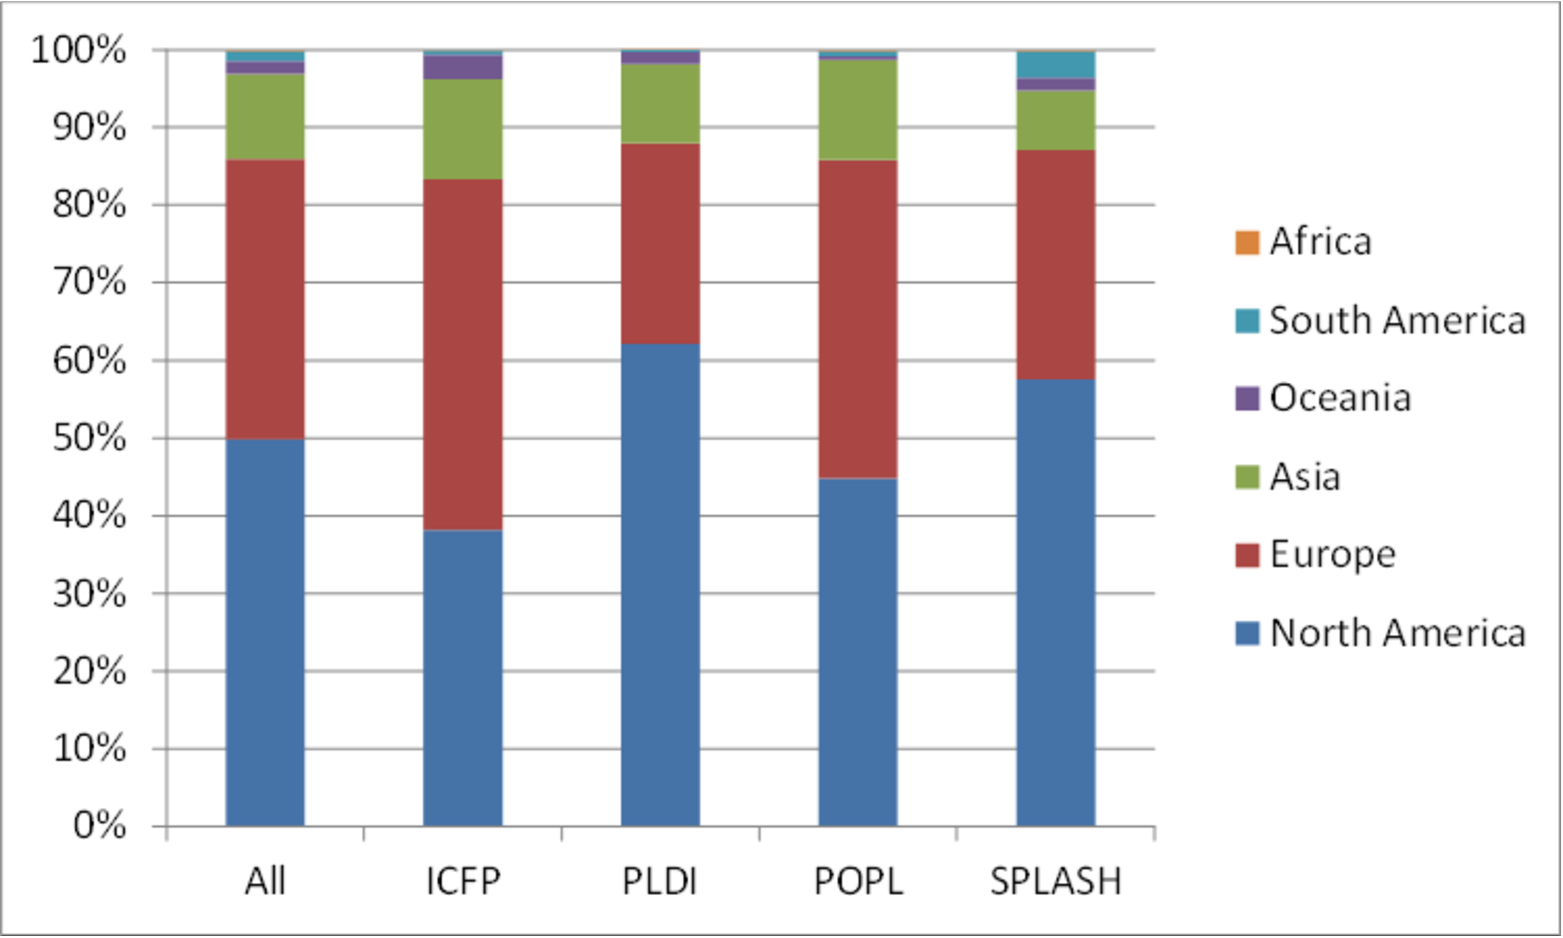
\includegraphics[width=0.7\textwidth]{ParticipantsOrigin.pdf}
  \caption{Overall origin of participants per conference.}
  \label{fig:demo-per-conf}
\end{figure}

\begin{table}
  \csvautotabular{../../output/sigplan/demographic_per_conf.csv}
\caption{For each kind of conference, distribution of participants per continent of origin}
\label{table:demo-per-conf}
\end{table}


Table~\ref{fig:demo-per-conf} and Figure~\ref{fig:demo-per-conf}\bcp{can we
  number tables and figures in the same sequence?} show where all
participants came from. For each conference, we depict the distribution of
attendance per continent. Table~\ref{fig:demo-per-conf} also shows the portion
of attendants originating from the same continent as the one the event took
place in. To a first approximation, maximizing this last metric, i.e. hosting
conferences in the continent containing the majority of its community, is a
first simple heuristic to consider.

Taken as a whole, these conferences attracted 50\% participants from North
America, 36\% from Europe, 11\% from Asia, 2\% from Oceania, 1\% from South
America, and less than 0.2\% from Africa.
This data also emphasizes the relative anchor to a specific continent each
conference may have.
Most notably, PLDI and SPLASH appear to be very North
American-centric, while ICFP's core community seems to have a quite strong
anchor in Europe as well.

\begin{table}
  \csvautotabular{../../output/sigplan/demographic.csv}
  \caption{For each \event, continent in which it took place and distribution of
    each continent by origin of participants. The final column indicates the
    portion of participants that traveled from the same continent the
    conference took place in.}
  \label{table:demo-per-event}
\end{table}

\begin{figure}
  \centering
  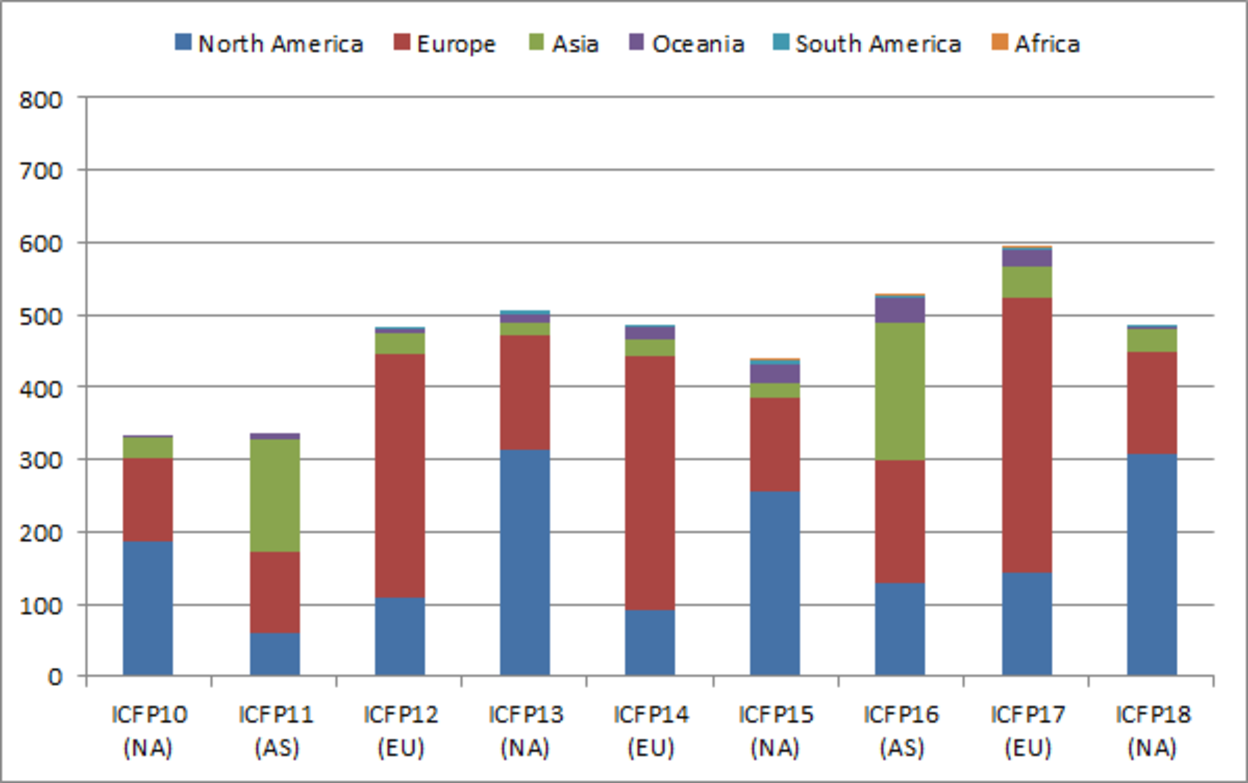
\includegraphics[width=0.45\textwidth,height=1.8in]{ParticipantsOriginICFP.pdf}
  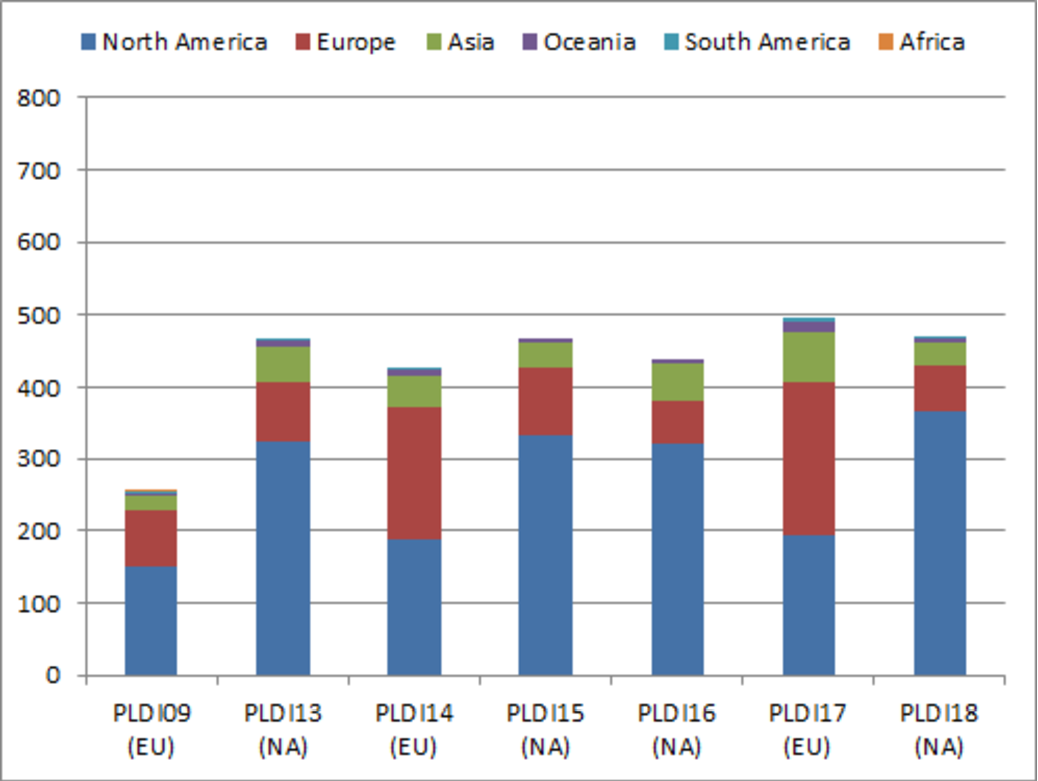
\includegraphics[width=0.45\textwidth,height=1.8in]{ParticipantsOriginPLDI.pdf}
  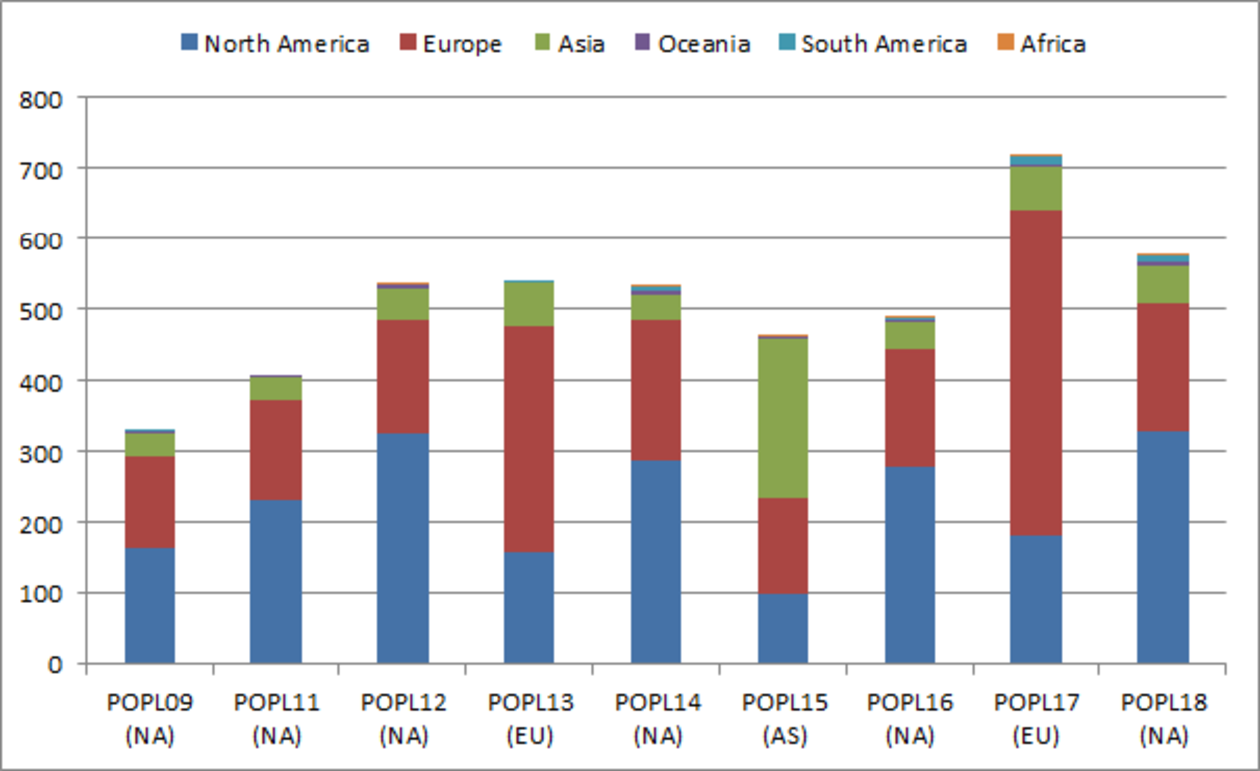
\includegraphics[width=0.45\textwidth,height=1.8in]{ParticipantsOriginPOPL.pdf}
  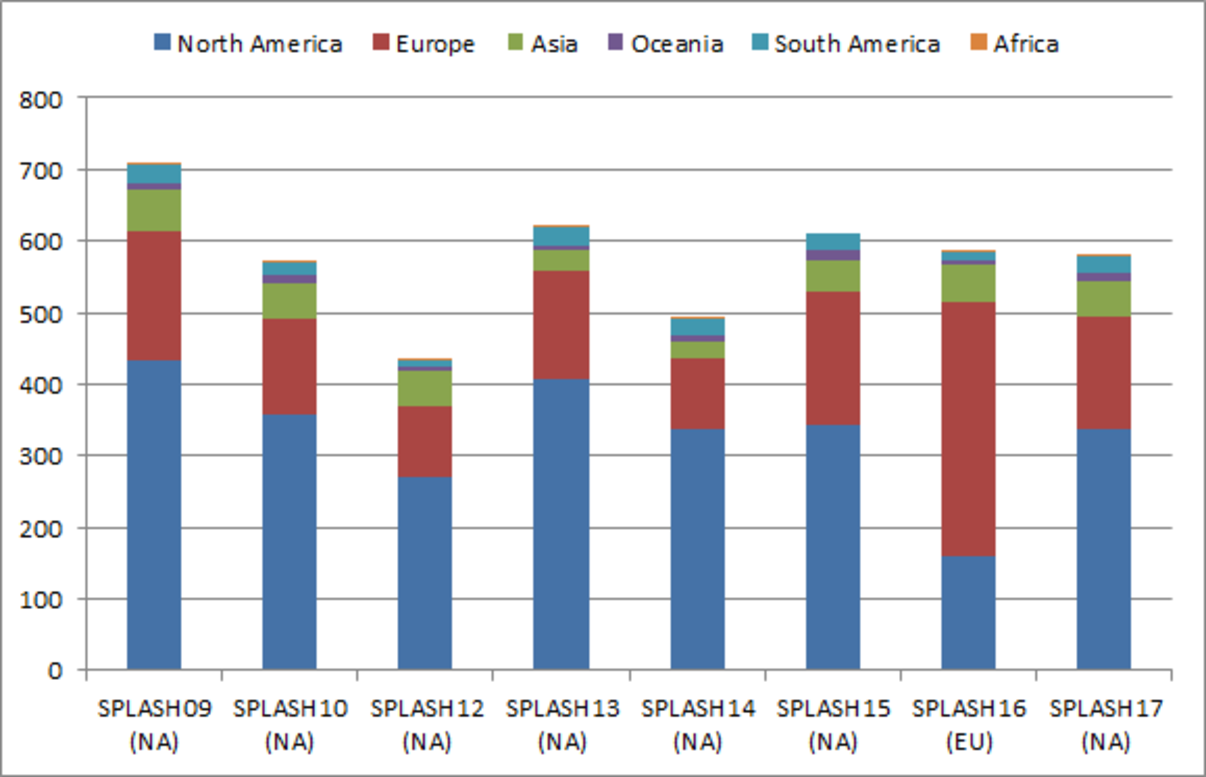
\includegraphics[width=0.45\textwidth,height=1.8in]{ParticipantsOriginSPLASH.pdf}
  \caption{Origin of participants for each conference, detail.}
  \label{fig:demo-per-event}
\end{figure}

This overall picture, however, hides some interesting facts pertaining to the
relationship between the conferences' locations and the origin of the participants.
Indeed, aggregating the attendance per conference intrinsically rests upon the
assumption of a uniform community attending each instance of the conference
every year. Table~\ref{fig:demo-per-event} and Figure~\ref{fig:demo-per-event}
show a more detailed breakdown of the origin of participants for each
conference, showing also the geographic region where the conferences were held.

These charts make it clear that the location of the conferences had a
substantial effect on attracting people from the same geographic areas. That
effect is quite visible for ICFP and POPL, with noticeable ups and downs of the
colored bars between North American and European participants when the
conferences were located in North America and Europe, respectively. Most
strikingly, Asian participation during POPL '15, ICFP '11 and ICFP '16, events
that took place on the Asian continent, is significantly higher than usual:
there appears to be a strong locality phenomenon. Crossing this data with
Table~\ref{table:footprint}, one can also notice that the only time SPLASH took
place in Europe turned out to be the least expensive edition, challenging our
previous observation that the conference appears to be mostly north
American-centric.

\begin{table}
  \csvautotabular{../../output/sigplan/demographic_delta.csv}
\caption{Geographical distribution of participation conditioned by the location of the \event}
\label{fig:local_effect}
\end{table}

Table~\ref{fig:local_effect} attempts to measure this locality effect. The
table depicts, all conferences being considered at once, the geographical
distribution of attendance conditioned by the geographical location of the
\event. The Asian phenomenon previously hinted at is here extremely
apparent: while overall on average, 10.9\% of the participants come from Asia,
this number is roughly multiplied by a factor 4 when the \event takes place in Asia --
without any significant drop in total volume of attendance that could indirectly bump
the percentage.
But interestingly, this phenomenon also exists in the case of Europe (+22.29\%
deviation to the average) and North America (+12.15\% deviation to the average).
Despite their name, international conferences appear to exhibit a fairly strong
local component.

Overall, this data shows that the goal of geographic inclusion was,
indeed, accomplished by organizing the conferences in diverse geographic areas
of the world. It also places Figure~\ref{fig:continents} into a broader context:
a naive interpretation of that chart might lead us to conclude that North
America and Europe are where most of this community is, but it is not that
simple. Because of the regional effect on participation, the distribution of
participants also reflects the fact that most of these conferences were held in
North America and Europe (30), only a few were held in Asia (3), and none was
held in South America, Oceania, or Africa.

The situation may be summed up into the following two elementary observations. 
\begin{obs}
  The vast majority of participants are split between North America and Europe,
  Asia to a much lesser degree. SPLASH and PLDI are strongly anchored in North
  America, ICFP and POPL fairly equally split between North America and Europe.
  \label{obs:dist-naive}
\end{obs}
This distribution however turns out to be \emph{strongly} dependent on the
location of the \event.
\begin{obs}
  There is a major ``locality" effect: it is both true that locality attract
  new participants, and distance repels some participants.
  \label{obs:locality}
\end{obs}

\subsection{How Often Did Participants Attend These Conferences?}
\label{subsec:overlap}

Section~\ref{subsec:demo}, through the study of the demographic distribution of
attendance, has suggested the existence of local communities that only
partake in conferences when they take place close to their place of residency.
One can conversely look for groups of regular attendees, that participate to a given \conf
regardless of the location it is held in.

\begin{figure}
  \centering
  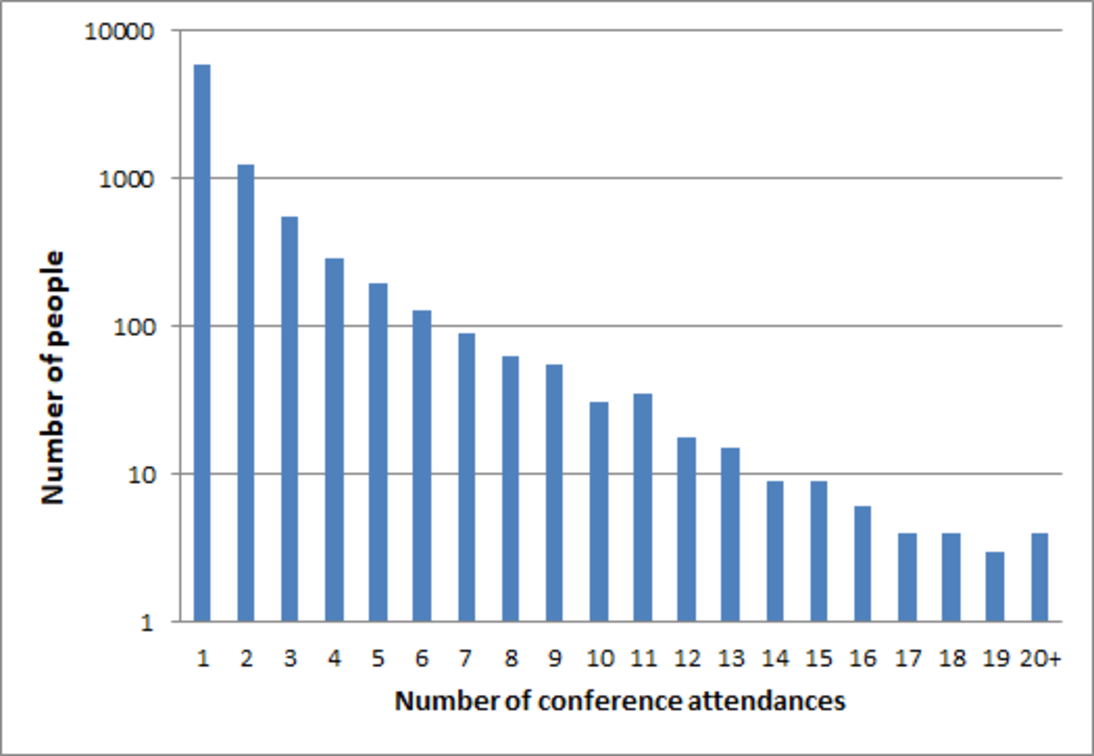
\includegraphics[width=0.6\textwidth]{AttendanceHist.pdf}
  \caption{Histogram of attendance.}
  \label{fig:hist_attendance}
\end{figure}

\begin{figure}
  \centering
  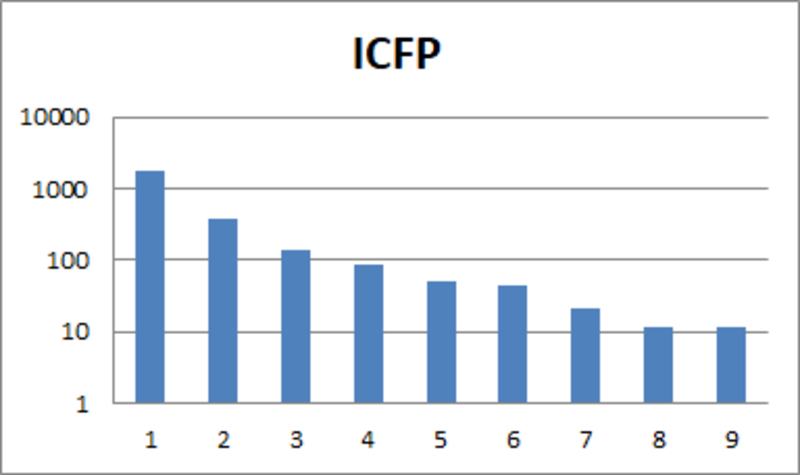
\includegraphics[width=0.45\textwidth,height=1.5in]{AttendanceHistICFP.pdf}
  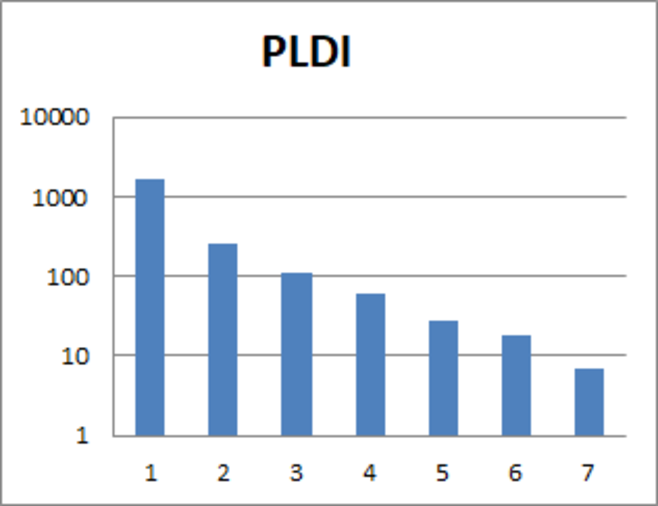
\includegraphics[width=0.4\textwidth,height=1.5in]{AttendanceHistPLDI.pdf}
  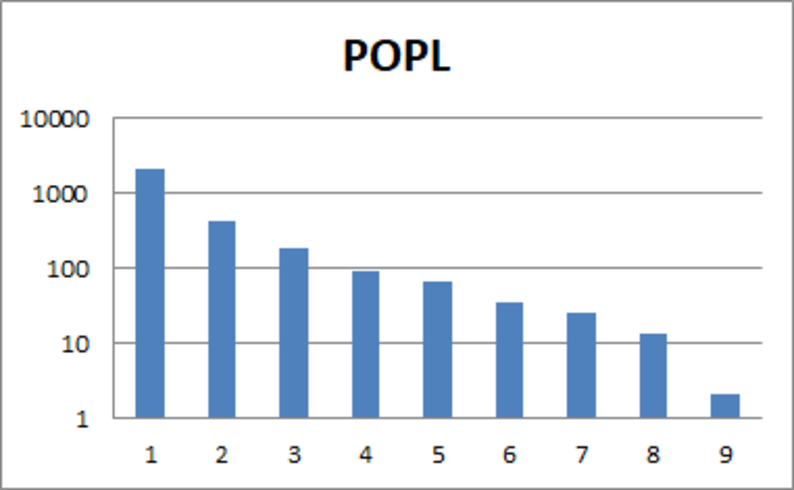
\includegraphics[width=0.45\textwidth,height=1.5in]{AttendanceHistPOPL.pdf}
  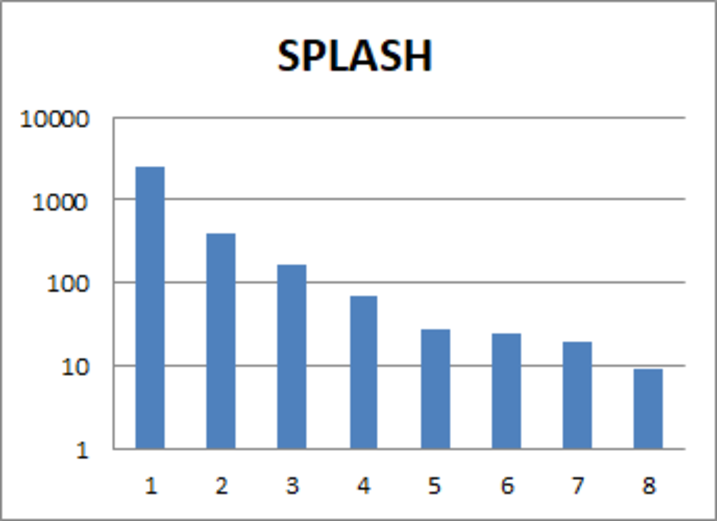
\includegraphics[width=0.4\textwidth,height=1.5in]{AttendanceHistSPLASH.pdf}
  \caption{Histogram of attendance for each conference series.}
  \label{fig:hist_attendance_per_conference}
\end{figure}

Figure~\ref{fig:hist_attendance} shows how often the same participants attended
multiple conferences. At the extremes, 6,009 people (69\%) attended only 1
conference, and 4 people attended 20 or more conferences. Participation is
dominated by single-conference participants, which reflects the large and
transient student population. The pattern is similar for each conference series,
shown in Figure~\ref{fig:hist_attendance_per_conference}.


\subsection{What Was the Participation Overlap Between These Conferences?}

We now take a closer look at the habits of these recurring participants.

\begin{figure}
  \centering
  \begin{subfigure}[b]{0.3\textwidth}
    \centering
    \csvautotabular{../../output/sigplan/overlap_cross_conf_ICFP_POPL.csv}
    \caption{POPL and ICFP}
  \end{subfigure}
  \begin{subfigure}[b]{0.3\textwidth}
    \centering
    \csvautotabular{../../output/sigplan/overlap_cross_conf_POPL_PLDI.csv}
    \caption{POPL and PLDI}
  \end{subfigure}
  \begin{subfigure}[b]{0.3\textwidth}
    \centering
    \csvautotabular{../../output/sigplan/overlap_cross_conf_POPL_SPLASH.csv}
    \caption{POPL and SPLASH}
  \end{subfigure}
  \begin{subfigure}[b]{0.3\textwidth}
    \centering
    \csvautotabular{../../output/sigplan/overlap_cross_conf_ICFP_PLDI.csv}
    \caption{ICFP and PLDI}
  \end{subfigure}
  \begin{subfigure}[b]{0.3\textwidth}
    \centering
    \csvautotabular{../../output/sigplan/overlap_cross_conf_ICFP_SPLASH.csv}
    \caption{ICFP and SPLASH}
  \end{subfigure}
  \begin{subfigure}[b]{0.3\textwidth}
    \centering
    \csvautotabular{../../output/sigplan/overlap_cross_conf_PLDI_SPLASH.csv}
    \caption{PLDI and SPLASH}
  \end{subfigure}
   \caption{For every year, overlap in attendance between the events of two
     different conferences\bcp{Maybe we could also have an aggregate count
       for each pair, showing how many people {\em ever} went to both (even
       in different years).}}
  \label{fig:overlap-cross}
\end{figure}

A first natural question is to ponder whether there is a significant overlap
in participation between conferences.
Figure~\ref{fig:overlap-cross} depicts for any pairing of the four
conferences considered the percentage of overlap. This measure is strikingly
low for most conferences.

\begin{obs}
  Cross-conference overlap is low: the tightest pairing sees slightly over 10\%
  of common attendance for a given year.  \bcp{More aggregated numbers would
  also be interesting, since I suspect that there are quite a few people
  that only go to one big conference a year, but may alternate between
  (e.g.) POPL and PLDI.}
  \label{obs:overlap-cross}
\end{obs}

\begin{table}
\centering
     \begin{subtable}[b]{0.4\textwidth}
       \centering
       \csvautotabular{../../output/sigplan/overlap_intra_conf_POPL.csv}
       \caption{Case of POPL}
     \end{subtable}
     \hfill
     \begin{subtable}[b]{0.4\textwidth}
       \centering
       \csvautotabular{../../output/sigplan/overlap_intra_conf_ICFP.csv}
       \caption{Case of ICFP}
    \end{subtable}

     \caption{For any two years, percentage of overlap in attendance at the corresponding editions of a conference (part 1)}
     \label{table:overlap-conf-alpha}
\end{table}

\begin{table}
\centering
     \begin{subtable}[b]{0.4\textwidth}
       \centering
       \csvautotabular{../../output/sigplan/overlap_intra_conf_PLDI.csv}
       \caption{Case of PLDI}
     \end{subtable}
     \begin{subtable}[b]{0.4\textwidth}
       \centering
       \csvautotabular{../../output/sigplan/overlap_intra_conf_SPLASH.csv}
       \caption{Case of SPLASH}
     \end{subtable}

     \caption{For any two years, percentage of overlap in attendance at the corresponding editions of a conference (part 2)}
     \label{table:overlap-conf-beta}
\end{table}

Conversely, one can estimate the overlap for a given conference over time.
Tables~\ref{table:overlap-conf-alpha}~and~\ref{table:overlap-conf-beta} depicts
for a given conference at a time, and for any pair of years, the percentage of
attendees that participated in both events. In particular for two consecutive
years, this number oscillate between 15\% and 30\%. The majority of
participants of a conference were therefore not part of the previous edition.

\begin{obs}
  Temporal overlap is moderate: roughly a quarter of attendants were present
  the year before at the same conference.
  \label{obs:overlap-temp}
\end{obs}

\begin{figure}
  \centering
  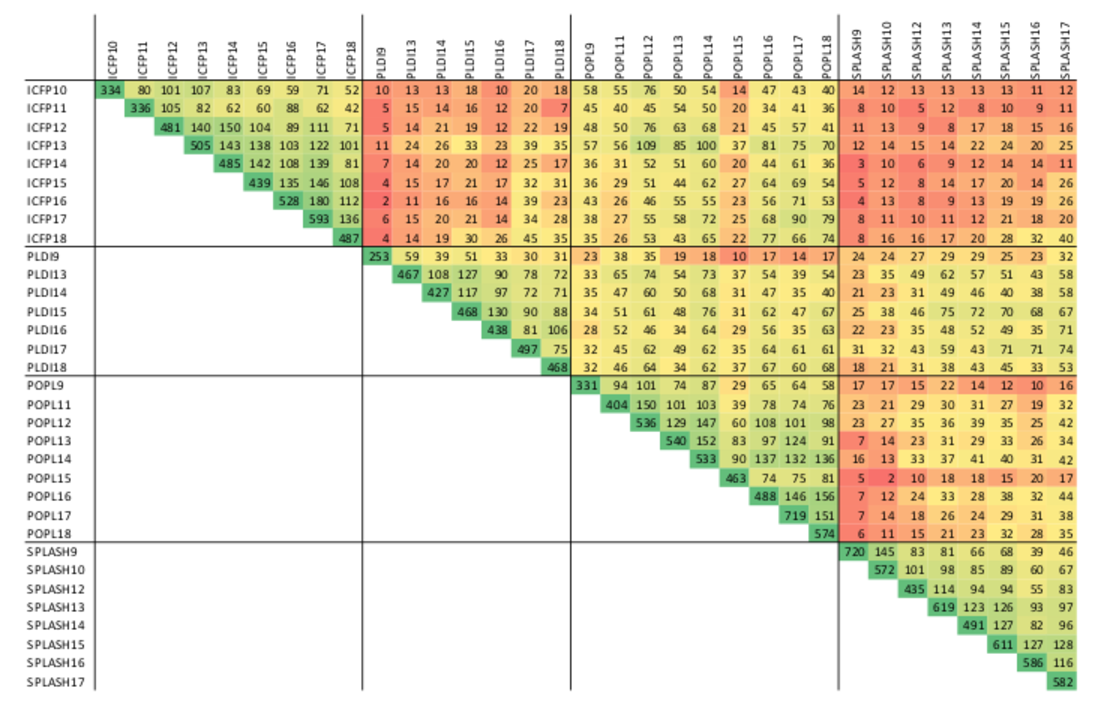
\includegraphics[width=\textwidth]{OverlapAnalysis-crop.pdf}
  \caption{Conference participation overlap.}
  \label{fig:overlap}
\end{figure}

Figure~\ref{fig:overlap} synthesizes these overlap in participants between the various
conferences, giving a bird-eye view of the permanence vs. transience of the
participants over time in SIGPLAN conferences. \yz{Should we scrap the three
  previous tables and only keep this Figure?}\bcp{I think so.}
In principle, it is desirable to
have a balance between repeat participants and newcomers. Communities that don't
attract new participants tend to stagnate; but communities that don't have a
core of repeat participants tend to lose focus.
\yz{Do we want to have this argument here?}\bcp{Sure, why not?}

The existence of a certain community associated with each conference series that
tends to repeat participation is clearly visible on the diagonal. The highest
overlap of all in particular was between ICFP'16 and ICFP'17, with 180
repeaters. The four conference series show a healthy balance between repeat
participation and newcomers.

The weaker overlap between conferences in different series is also apparent.
For example, there is a somewhat surprising overlap between PLDI and
POPL, followed by ICFP and POPL and by PLDI and SPLASH. The weakest overlaps are
between ICFP and SPLASH, followed by ICFP and PLDI, and by POPL and SPLASH. It
is unclear whether the overlap, or lack thereof, between these conference series
is due to intellectual reasons or due to their dates. PLDI and POPL is the pair
that is most distant in time, typically June and January, respectively. ICFP and
SPLASH is the pair that is the closest in time, typically September and October.
Time proximity may detract cross-participation.

\begin{table}
  \csvautotabular{../../output/sigplan/number_of_participations.csv}
\caption{Overall and for each conference, the average number of instances a
  participant has taken part of, and the percentage of them that has
  attended at least $k$ instances, for $k\in\llbracket 2 \dots 5
  \rrbracket$. Remark: the means and percentages are here computed with
  respect to \emph{unique} participants.  \bcp{I really like this table.}}
\label{table:reccurent}
\end{table}

\begin{table}
  \centering
  \begin{subtable}[b]{0.4\textwidth}
    \centering
    \csvautotabular{../../output/sigplan/old_timer_POPL.csv}
    \caption{Case of POPL}
  \end{subtable}
  \begin{subtable}[b]{0.4\textwidth}
    \centering
    \csvautotabular{../../output/sigplan/old_timer_ICFP.csv}
    \caption{Case of ICFP}
  \end{subtable}
  \\
  \begin{subtable}[b]{0.4\textwidth}
    \centering
    \csvautotabular{../../output/sigplan/old_timer_PLDI.csv}
    \caption{Case of PLDI}
  \end{subtable}
  \begin{subtable}[b]{0.4\textwidth}
    \centering
    \csvautotabular{../../output/sigplan/old_timer_SPLASH.csv}
    \caption{Case of SPLASH}
  \end{subtable}
  \caption{For each conference, percentage of participants that have been
    part of a previous edition of the same conference \bcp{Is this sort of
      the same information as Table 8?}}
  \label{table:old-timers}
\end{table}

Finally, Table~\ref{table:reccurent} and \ref{table:old-timers} offer two
different views on reccurent participations. Table~\ref{table:reccurent}
represents respectively for the whole dataset and for each conference
individually the average number of editions an average participant has been part
of, as well as the percentage of participants that has been part of at least
some amount of times. We immediately remark that no less than 75\% of unique
participants has been part of a single edition. Table~\ref{table:old-timers}
represents for each instance of each conference the percentage of participants
that has participated in a previous instance of the conference, among our
dataset.

\begin{obs}
  The average amount of conferences a participant has been part of is extremely low: 1.52.
  Less than 4\% of unique participants have been to more than five events
  among our dataset\bcp{Is that an accurate way of saying it?  I thought it
    was ``have been to five instances of the same conference.''  (The other
    number would be interesting too---how many people went to 2,3,4,5
    instances of {\em any} of the conferences?}\yz{We have both data. This
    observation refers 
    to the line ``ALL'' from Table 7}.\bcp{Maybe we can state it more
    clearly to avoid my confusion?}
  Similarly, at any \event, more than half of the participants are experiencing this specific
  conference for the first time.
  \label{obs:old-timers}
\end{obs}


